\documentclass[a4paper,11pt]{article}

\usepackage[T1]{fontenc}
\usepackage{lmodern}
\usepackage[dutch]{babel}
\usepackage{geometry}
\usepackage{microtype}
\usepackage{icomma}
\usepackage{booktabs}
\usepackage{array}
\usepackage{graphicx}
\usepackage{float}
\usepackage{amsmath}
\usepackage{hyperref}
\usepackage{titlesec}

\geometry{top=1.50cm,bottom=1.50cm,left=1.85cm,right=1.85cm}
\hypersetup{colorlinks=true,linkcolor=black,urlcolor=blue}
\linespread{1.03}
\setlength{\parindent}{0pt}
\setlength{\parskip}{5pt plus 0.8pt minus 0.5pt}
\setlength{\textfloatsep}{10pt plus 2pt minus 1pt}
\setlength{\floatsep}{10pt plus 2pt minus 1pt}
\setlength{\intextsep}{10pt plus 2pt minus 1pt}
\setlength{\abovecaptionskip}{5pt}
\setlength{\belowcaptionskip}{3pt}
\setcounter{secnumdepth}{3}
\titleformat{\section}{\large\bfseries}{\thesection}{0.5em}{}
\titleformat{\subsection}{\normalsize\bfseries}{\thesubsection}{0.45em}{}
\titleformat{\subsubsection}{\normalsize\bfseries}{\thesubsubsection}{0.4em}{}
\titlespacing*{\section}{0pt}{10pt plus 2pt minus 1pt}{5pt}
\titlespacing*{\subsection}{0pt}{8pt plus 2pt minus 1pt}{4pt}
\titlespacing*{\subsubsection}{0pt}{7pt plus 1pt minus 1pt}{3pt}

\newcommand{\dist}{\ensuremath{D}}

\begin{document}
\raggedbottom

\begin{center}
  {\LARGE\bfseries Order batching bij Optioryx}\\[3pt]
  {\large Retrospectieve experimentele analyse}\\[5pt]
  {Ze Ip \enspace--\enspace 02006554}
\end{center}
\vspace{4pt}

\textbf{Evaluatieprotocol.} De instantie bevat $10\,246$ orders in twaalf
waves. Een route bevat maximaal $n_{\max}=20$ orders uit één wave, splitst geen
order en volgt START--unieke picklocaties in snake-volgorde--END. De
doelfunctie \dist{} is de som van alle routeafstanden. De gecontroleerde
Release-tijdstudies liepen
serieel op een Intel Core i7-8750H met GCC~13.2, een Release-build en
\texttt{-O3}. Configuraties en seeds werden waar mogelijk in vergrendelde,
gerandomiseerde volgorde uitgevoerd. In de stochastische
volledige-instantieanalyses vormen de twaalf opgetelde waves per seed één
waarneming. Hun gemiddelden, steekproef-SD en tweezijdige
Student-$t$-95\%-betrouwbaarheidsintervallen gebruiken de tien gekoppelde seeds
0--9. Holm-correctie gebeurt per vooraf bepaalde familie.
Gelijke seedlabels maken gekoppelde contrasten mogelijk, al kan een
factorwijziging het verdere
verbruik van toevalsgetallen veranderen. Afzonderlijke protocollen worden niet
samengevoegd.

\section{Metaheuristieken}

\subsection{Greedy heuristiek}
Elke order start als afzonderlijke route. Het haalbare paar met maximale
besparing $s(A,B)=C(A)+C(B)-C(A\cup B)$ wordt samengevoegd. Hier is $C$ de
exacte snake-routekost over unieke locaties. Een prioriteitswachtrij met
uitgestelde actualisatie beperkt herberekening. Daarna worden routes volgens
het middelpunt van hun snake-span gesorteerd. Eén passage onderzoekt elk
routepaar binnen een venster van acht. Per paar wordt herhaald de beste strikt
verbeterende swap of capaciteitsgeldige relocate toegepast totdat geen van
beide nog verbetert. Lege routes verdwijnen. Deze LS1 vormt de
gemeenschappelijke basis voor de gecontroleerde vergelijking. Uitgebreidere
route-eliminatie en heropbouw worden afzonderlijk onderzocht, omdat hun veel
grotere budget niet uitwisselbaar is met dat van de LS1-basis.
Bij eliminatie herverdeelt een begrensde beamzoektocht alle orders van een bronroute
over vrije capaciteit. Pair- en triple-rebuild combineren twee of drie nabije
routes en proberen deterministische volledige herpartitioneringen. Alleen
strikt goedkopere uitkomsten worden behouden.
De grootste onmiddellijke besparing is aannemelijk wanneer ruimtelijk
overlappende orders ook samen een goede batch vormen. De keuze kijkt echter
niet vooruit. Een vroege samenvoeging kan daardoor latere, betere combinaties
blokkeren. LS1 herstelt een deel van zulke fouten, maar alleen binnen het
beperkte routevenster.

\subsection{Simulated annealing}
Het volledige $2\times2\times2$-ontwerp combineert geometrische of
Lundy--Mees-koeling, \emph{relocate} of \emph{swap} en een greedy-LS1-start of
een willekeurige start. Beide buurten bewaren wave en capaciteit. Iedere run
gebruikt 400 iteraties met $T_0=60$ en $T_f=0,05$. De willekeurige start schudt
de orders per wave en verdeelt ze daarna in volle batches van twintig, gevolgd
door hoogstens één restbatch. Deze capaciteitsvullende randomstart gebruikt dus
de routeondergrens van 517. De greedy-LS1-start telt 534 routes. Geometrische koeling gebruikt
$T_{k+1}=\max(T_f,\alpha T_k)$. Lundy--Mees gebruikt
$T_{k+1}=T_k/(1+\beta T_k)$. De factoren worden zo bepaald dat beide schema's
dezelfde begin- en eindtemperatuur delen.
Relocate verplaatst één order naar een bestaande niet-volle of een nieuwe
singletonroute. Een lege bronroute verdwijnt, waardoor het routeaantal kan
stijgen of dalen. Swap wisselt orders tussen twee routes en bewaart hun groottes
en het routeaantal. Zo contrasteert een flexibele bezettingswijziging met een
beweging die ook bij volledig gevulde routes toepasbaar blijft.

Na Holm-correctie zijn start, buurt en hun interactie aantoonbaar. Tegenover de
greedy-start verhoogt randomisatie \dist{} gemiddeld met
$5\,450\,754$ [95\%-BI $5\,442\,863$--$5\,458\,644$]. Swap verlaagt \dist{}
gemiddeld met $204\,702$ [197\,448--211\,956], maar bijna het volledige effect
ontstaat bij randomstarts. Het koelschema geeft slechts $-744$
[$-9\,200$--$7\,712$] en blijft na correctie niet aantoonbaar. De startstrategie
is binnen 400 stappen dus belangrijker dan de keuze tussen deze koelschema's.
Ze verandert echter tegelijk samenstelling en routeaantal, zodat die twee
effecten niet afzonderlijk identificeerbaar zijn. Dat de randomstart ondanks
517 routes veel slechter is, toont wel dat minimaal routeaantal alleen niet
volstaat. De volledige cellen en contrasten staan in
Tabel~\ref{tab:app-sa} en Tabel~\ref{tab:app-sa-effects}.

\subsection{Genetisch algoritme}
Een chromosoom is per wave een orderpermutatie. Een dynamische decoder kiest de
optimale opeenvolgende batches van maximaal twintig orders, zodat elk chromosoom
haalbaar decodeert. Eén greedy-LS1-permutatie bewaart startkwaliteit. De overige
individuen zijn willekeurig. De basis gebruikt populatie 12, twintig generaties,
toernooigrootte 3, order crossover, mutatiekans 0,20, een gelijke mix van
invoeg- en wisselmutatie conditioneel op een mutatie en elitisme 0,08. Fitness
rangschikt haalbaar gedecodeerde oplossingen op de laagste totale afstand.

Geen van acht gekoppelde OFAT-kwaliteitscontrasten blijft significant na Holm-
correctie. Populatie 24 geeft bijvoorbeeld $\Delta D=-243$
[$-478$--$-9$], maar $p_{\mathrm{Holm}}=0,347$. De gemiddelde genormaliseerde
Hammingdiversiteit van de basis daalt van 0,997 naar 0,109. Een mutatiekans van
0,40 verhoogt de einddiversiteit tot 0,221 zonder aantoonbare kwaliteitswinst.
De decoder maakt batchgrenzen impliciet in aaneengesloten chromosoomsegmenten.
Kruising en positieveranderingen kunnen daardoor nuttige lokale
batchstructuren verbreken. Samen met de snelle homogenisering vormt dit een
plausibele verklaring voor de beperkte winst. De OFAT-conclusies blijven conditioneel op de vaste operatoren
en identificeren geen interacties. Tabel~\ref{tab:app-ga} geeft alle acht
varianten.

\subsection{Vergelijkende studie}
De gecontroleerde Release-studie gebruikt dezelfde deterministische
greedy-LS1/venster-8-oplossing als referentie en sterke start. SA gebruikt
geometrische koeling, relocate, $T_0=60$ en $T_f=0,05$. De koelfactor wordt per
iteratiebudget herberekend, zodat alle budgetten dezelfde eindtemperatuur
bereiken. GA gebruikt de hierboven beschreven basis en varieert alleen het
aantal generaties. De uitvoeringsvolgorde van acht configuraties en tien seeds
is per wave gerandomiseerd. Alle 960 wave-runs waren haalbaar.

\begin{table}[H]
\centering
\small
\setlength{\tabcolsep}{3.5pt}
\begin{tabular}{@{}lrrlr@{}}
\toprule
\textbf{configuratie} & \textbf{$\bar D\pm$SD} & \textbf{$\bar t\pm$SD (s)} &
\textbf{winst [95\%-BI] (\%)} & \textbf{$p_{\rm Holm}$} \\
\midrule
greedy LS1 & $5\,307\,302\pm0$ & $12,057\pm0,367$ & 0 & --- \\
SA, $10\,000$ iter. & $5\,301\,464\pm1\,789$ & $13,195\pm0,555$ & $0,1100\,[0,0859\text{--}0,1341]$ & $<0,001$ \\
GA, 40 gen. & $5\,307\,044\pm182$ & $31,148\pm1,823$ & $0,0049\,[0,0024\text{--}0,0073]$ & 0,008 \\
\bottomrule
\end{tabular}
\caption{Beste onderzochte budget per algoritme in de gecontroleerde studie
met tien gekoppelde seeds. Afstand en interne solvertijd zijn per seed over
twaalf waves gesommeerd. Positieve winst is beter dan greedy. Holm corrigeert
gezamenlijk over alle zeven stochastische budgetpunten. De volledige
budgetreeks staat in Figuur~\ref{fig:comparison} en
Tabel~\ref{tab:app-budget}.}
\label{tab:comparison}
\end{table}

\subsubsection{Uitvoeringstijd}
De schaalstudie gebruikt binnen W000003 drie willekeurige geneste subsetreeksen
met achtereenvolgens 50, 100, 200, 400 en 800 orders, drie seeds en dezelfde subsets voor elke
methode. Dit levert 135 seriële runs op. OLS op de logaritme van de mediane
interne tijd schat $T(n)=an^b$. De exponenten met Student-$t$-95\%-BI zijn
1,888 [1,810--1,967] voor greedy, 1,892 [1,842--1,942] voor SA en 1,303
[1,176--1,429] voor GA. Met vast $n_{\max}=20$ is de bijna-kwadratische groei
van greedy verenigbaar met routepaarinitialisatie. SA bevat dezelfde start en
een vast iteratiebudget. GA combineert die ene kwadratische warmstart met een
evolutieve decoder die $O(PG\,n\,n_{\max})$ kandidaatsegmenten test. De werkelijke
tijd omvat ook het scoren ervan. De GA-exponent beschrijft daarom een
gemengd eindig bereik en geen asymptotische complexiteit. De tijdsniveaus staan
in Tabel~\ref{tab:app-scaling}.

\begin{figure}[H]
\centering
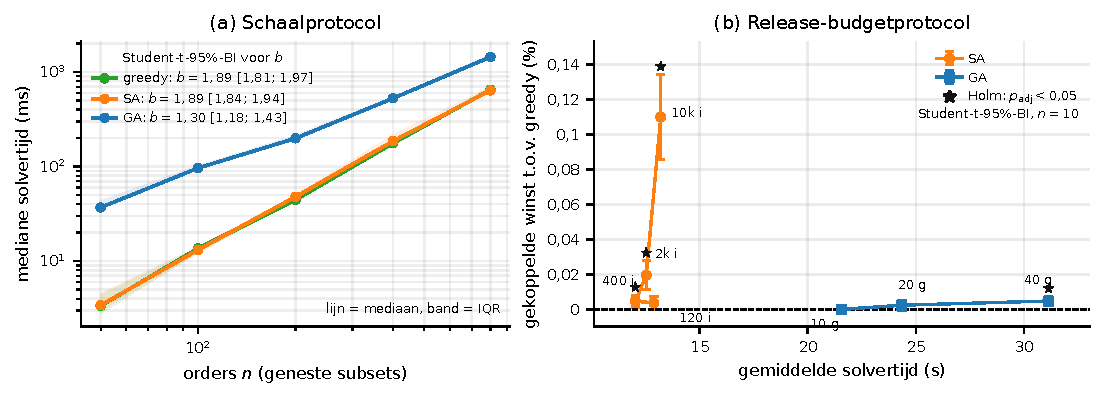
\includegraphics[width=0.98\linewidth]{figures/retrospective_comparison.pdf}
\caption{Gecontroleerde vergelijking. (a) Mediane interne tijd en IQR op
geneste subsets, met Student-$t$-95\%-BI voor de schaalexponent. (b) Gemiddelde
gekoppelde afstandswinst en 95\%-BI per Release-budget. Sterren markeren
Holm-significantie binnen de zeven budgettoetsen.}
\label{fig:comparison}
\end{figure}

\subsubsection{Convergentie}
Een afzonderlijke studie registreert voor tien seeds de volledige best-so-far-
curve. De som over waves bij hetzelfde stapnummer is een gesynchroniseerde
werkbudgetcurve en geen chronologische tijdlijn. $t_{95}$ en $t_{99}$ gelden
alleen ten opzichte van de uiteindelijke winst binnen het eigen budget. De
budgetcontrast-BI's zijn ongecorrigeerde Student-$t$-intervallen. Bij
SA-10\,000 ligt de mediane $t_{95}$ op $9\,259$ en $t_{99}$ op
$9\,415$ iteraties. Bij SA-50\,000 worden dit $42\,872$ en $47\,924$. Alle
twintig SA-runs verbeteren nog in de laatste 10\% van hun budget. SA-50\,000
verbetert tegenover de alternatieve 10\,000-configuratie gemiddeld nog
$13\,606$ [95\%-BI $12\,071$--$15\,141$], bij een gemiddelde tijdsratio van
1,184. Beide budgetten gebruiken echter een eigen koelfactor tot hetzelfde
$T_f$ en zijn dus geen voortgezette curve. Binnen de gemeten horizon is voor SA
geen plateau aangetoond.

GA gebruikt één RNG-stroom opeenvolgend over de waves. Een ander
generatiebudget verschuift daardoor na de eerste wave de RNG-toestand. De drie
horizonten zijn dus afzonderlijke uitvoeringen met dezelfde seedlabels. Bij GA-200 geeft één seed
geen winst. Voor de negen verbeterende seeds vallen de mediane $t_{95}$ en
$t_{99}$ beide op generatie 164 [IQR 145--172]. Slechts één seed verbetert nog
in de laatste 10\% en geen op generatie 200. De stap van 100 naar 200 generaties
levert gemiddeld $538$ [$-113$--$1\,189$] bij 1,666 keer de tijd. Dit wijst op
afnemende meeropbrengst, maar bewijst geen volledig plateau.

\begin{figure}[H]
\centering
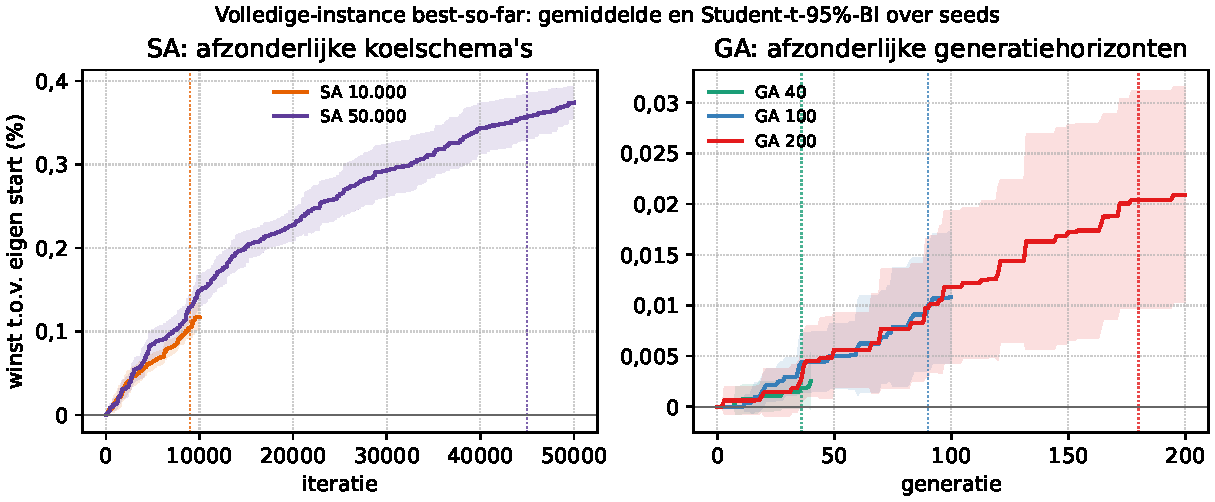
\includegraphics[width=0.96\linewidth]{figures/retrospective_long_convergence.pdf}
\caption{Lange convergentie met tien seeds per budget. Curven tonen gemiddelde
winst tegenover de eigen start met ongecorrigeerde Student-$t$-95\%-BI's. De
stippellijnen markeren 90\% van elk budget. SA-budgetten gebruiken afzonderlijke
koelschema's. GA-horizonten zijn geen gedeelde volledige-instanceprefixen.}
\label{fig:long-convergence}
\end{figure}

\subsubsection{Verschillen tussen de waves}
SA-10\,000 verbetert in minstens één seed bij elf van twaalf waves. Acht ruwe
intervallen sluiten nul positief uit. Na Holm-correctie over twaalf waves
blijven W000002, W000005, W000007 en W000010 significant. GA-40 verbetert in
minstens één seed bij vijf waves, maar geen wave blijft significant. De grootste
relatieve SA-puntschatting ligt bij de kleine W000011 en is door seedspreiding
niet Holm-significant. Een enkel wavekenmerk volstaat dus niet als verklaring.
Vooraf gekozen verklarende kenmerken waren orderaantal, gemiddelde paarsgewijze
Jaccard-overlap van unieke picklocaties en de SD van orderspans. Exploratief
correleert alleen de relatieve GA-winst aantoonbaar negatief met orderaantal
($\rho=-0,773$, $p_{\mathrm{Holm}}=0,0095$), maar twaalf waves met veel
nulwaarden laten geen causale conclusie toe. De wavegewijze contrasten staan in
Tabel~\ref{tab:app-waves}.

\subsubsection{Rekentijd versus kwaliteit}
SA-400 meet gemiddeld 12,016 s tegenover 12,057 s voor greedy ($-0,35\%$) en
geeft een kleine Holm-significante winst. De extra winst van SA-2\,000 tegenover SA-400 bedraagt
$789$ [431--$1\,146$]. SA-10\,000 voegt daar nog $4\,796$
[$3\,784$--$5\,807$] aan toe en kost gemiddeld slechts 9,44\% meer tijd dan
greedy. GA-40 verbetert tegenover GA-20 met $127$ [18--236], maar kost 2,58 keer
de greedytijd en blijft slechter dan SA-10\,000. Binnen deze budgetten domineert
SA daarom de gemeten GA-keuzes op zowel tijd als kwaliteit.

\subsubsection{Zelfgekozen bijkomende analyse}
Het cumulatieve greedy-ontwikkelingspad start op $D=5\,511\,080$ met 534 routes.
Lokale paarzoektocht verlaagt dit naar $5\,100\,290$ en levert 72,1\% van de
uiteindelijke winst. De gebundelde fase eliminatie en post-LS bereikt vervolgens
de ondergrens van 517 routes. Gebundelde pair-, triple- en combinatiestappen eindigen op
$D=4\,941\,530$, een totale reductie van 10,33\%. Dit pad is geen causale
ablatie. Fasen bundelen meerdere wijzigingen, afstanden zijn historische
afgeronde scores en elke tijd is één meting. Bovendien vonden ontwikkeling en
selectie adaptief op dezelfde instantie plaats zonder testinstantie. De $2\,523$ s
voor het eindpunt is daarom alleen een orde van grootte.
Tabel~\ref{tab:app-greedy} documenteert de afzonderlijke mijlpalen.

\section{Probleemspecifieke heuristieken}

\subsection{Beschrijving van de heuristieken}
De rechthoekige dekkingsregels uit de opdracht worden aangepast aan de vaste
snake-route. \emph{Smallest} en \emph{greatest rectangular covering area}
worden respectievelijk de kleinste en grootste span tussen de uiterste
snake-ranks van een order. \emph{Greatest number of identical picking
locations} maximaliseert locatieoverlap. \emph{Smallest additional covering
area} minimaliseert de extra span na toevoeging aan de huidige batch. Gelijke
seedscores behouden de invoervolgorde. Bij selectieties volgt incrementele kost
op overlap of spanuitbreiding, terwijl span volgt op incrementele kost. Verdere
ties behouden de invoervolgorde. Iedere batch wordt tot maximaal twintig orders gevuld.
De twee extreme spanseeds toetsen of een compacte of juist brede eerste order
gunstiger is. De selectieregels contrasteren hergebruik van dezelfde locaties
met het begrenzen van de extra route-omvang.

\subsection{Invloed van seed- en selectieregel}
In het deterministische $2\times2$-experiment verlaagt minimale spanuitbreiding
het gemiddelde van 7,604 naar 6,798 miljoen, een winst van 10,60\% tegenover
maximale overlap. De grootste-spanseed verlaagt het gemiddelde met 157\,464 of
2,16\% tegenover de kleinste-spanseed. Het selectiecontrast van 806\,285 is dus
5,1 keer groter dan het seedcontrast. De beste oorspronkelijke combinatie is
grootste span met minimale spanuitbreiding op $D=6\,759\,161$. Alle
regelcombinaties staan in Tabel~\ref{tab:app-seed}.

\subsection{Prestatievergelijking met greedy heuristiek}
De beste oorspronkelijke combinatie blijft 27,36\% boven de gecontroleerde
greedy-LS1-score. Haar mediane interne tijd bedraagt 6,681 s tegenover 12,057 s
voor greedy. Deze tijden komen uit afzonderlijke Release-protocollen en vormen
daarom slechts een beschrijvende vergelijking. Minimale directe routekost met
de kleinste-spanseed verkleint de kwaliteitsachterstand tot 3,39\% bij een
mediaan van 6,880 s.

\subsection{Ontwerp van een eigen regel}
De begrensde tweestapsvooruitblik selecteert eerst de $K$ laagste directe
meerkosten. Voor elke eerste kandidaat wordt de goedkoopste haalbare tweede
toevoeging gezocht. De kandidaat met het beste tweestapsresultaat wordt gekozen.
De score gebruikt de exacte snake-routekost en de capaciteit van twintig
orders. Alleen de eerste kandidaat wordt definitief toegevoegd. De tweede dient
uitsluitend als vooruitblik. Hierdoor blijft de stapkost begrensd, terwijl een
eerste keuze die pas na de volgende order gunstig wordt zichtbaar kan blijven.

Voor $K\in\{2,4,8,16\}$ is de volledige deterministische configuratie telkens
tienmaal in gerandomiseerde volgorde gemeten. De score was binnen elke
configuratie exact identiek. Met de kleinste-spanseed is $K=8$ het beste punt:
$D=5\,436\,249$, of 0,928\% beter dan directe kost. De mediane tijd stijgt van
6,880 s naar 41,075 s, een factor 5,97. $K=16$ is met 77,380 s trager en met
0,723\% winst slechter. Voor de grootste-spanseed is $K=8$ eveneens het beste
kwaliteitsresultaat met 1,133\% winst. Kwaliteit verbetert dus niet monotoon met
$K$.

\subsection{Rekentijd versus kwaliteit}
De originele span- en overlapregels zijn snel, maar leveren 27\% of meer
kwaliteitsverlies tegenover greedy. Tweestapsvooruitblik sluit een deel van die
kloof, maar $K=8$ met de kleinste-spanseed blijft 2,43\% slechter en de mediane
41,075 s ligt ruim boven de afzonderlijk gemeten greedytijd. Het punt wordt in
deze beschrijvende vergelijking dus door greedy gedomineerd. Een kleine $K$ is
alleen verdedigbaar wanneer de eenvoudige constructieregel zelf vereist is.

\subsection{Kritische analyse}
De constructie is onomkeerbaar en corrigeert geen vroege batchfout. De
spanvertaling verliest tweedimensionale geometrie en ordercapaciteit geeft andere
prikkels dan itemcapaciteit. De $K$-voorselectie kan de beste eerste keuze
uitsluiten, terwijl grotere $K$ geen monotone kwaliteitswinst geeft. Eén
instantie ondersteunt geen generaliseerbaarheid.

\textbf{Besluit.}
SA-400 biedt rond twaalf seconden een kleine aantoonbare winst boven LS1-greedy.
In de gecontroleerde budgetstudie geeft SA-10\,000 bij dertien seconden 0,1100\%
winst voor 9,44\% extra tijd. De lange studie vindt nog geen SA-plateau en geen
zekere meerwinst van GA-100 naar GA-200. Zonder strak tijdbudget bereikt de
adaptieve greedy-pijplijn $D=4\,941\,530$, maar één tijdmeting en geen
testinstantie verhinderen robuuste runtime- en generalisatieclaims. De
tweestapsregel verbetert de eenvoudige constructie, maar blijft door LS1-greedy
gedomineerd.

\clearpage
\appendix
\numberwithin{table}{section}
\numberwithin{figure}{section}
\section{Factorieel en OFAT-onderzoek}
\label{app:meta}

\begingroup
\footnotesize
\setlength{\tabcolsep}{2.5pt}
\setlength{\intextsep}{5pt}
\setlength{\abovecaptionskip}{3pt}
\setlength{\belowcaptionskip}{2pt}
\renewcommand{\arraystretch}{0.96}

\begin{table}[H]
\centering
\caption{Volledig $2\times2\times2$-SA-ontwerp met een capaciteitsvullende
randomstart. Voor elke seed zijn $D$ en de interne solvertijd over de twaalf
waves opgeteld. De resultaten zijn gebaseerd op tien gekoppelde seeds.}
\label{tab:app-sa}
\begin{tabular}{@{}lllrrr@{}}
\toprule
\textbf{start} & \textbf{koeling} & \textbf{buurt} &
\textbf{$\bar D\pm$SD} & \textbf{beste $D$} & \textbf{$\bar t$ (s)} \\
\midrule
greedy & geometrisch & relocate & $5\,308\,303\pm458$ & $5\,307\,359$ & $12,179$ \\
greedy & geometrisch & swap     & $5\,307\,697\pm527$ & $5\,306\,678$ & $12,219$ \\
greedy & Lundy--Mees & relocate & $5\,308\,154\pm441$ & $5\,307\,423$ & $13,174$ \\
greedy & Lundy--Mees & swap     & $5\,307\,592\pm450$ & $5\,306\,974$ & $12,079$ \\
\midrule
willekeurig & geometrisch & relocate & $10\,956\,014\pm22\,702$ & $10\,917\,264$ & $0,028$ \\
willekeurig & geometrisch & swap     & $10\,562\,728\pm18\,863$ & $10\,538\,780$ & $0,027$ \\
willekeurig & Lundy--Mees & relocate & $10\,970\,186\pm8\,831$  & $10\,957\,547$ & $0,027$ \\
willekeurig & Lundy--Mees & swap     & $10\,545\,832\pm29\,989$ & $10\,501\,489$ & $0,028$ \\
\bottomrule
\end{tabular}
\end{table}

\begin{table}[H]
\centering
\caption{Gekoppelde SA-effecten op $D$. De Student-$t$-95\%-BI's zijn
ongecorrigeerd. De kolom $p_{\mathrm H}$ bevat de Holm-gecorrigeerde $p$-waarden voor
zeven toetsen. De contrasten zijn $K$: Lundy--Mees min geometrisch, $B$: swap
min relocate en $S$: willekeurig min greedy. Een positieve $\Delta D$ is
ongunstig.}
\label{tab:app-sa-effects}
\begin{tabular}{@{}lrr@{}}
\toprule
\textbf{effect} & \textbf{$\Delta D$ [95\%-BI]} & \textbf{$p_{\mathrm H}$} \\
\midrule
$K$             & $-744\;[-9\,200\text{--}7\,712]$ & $1,000$ \\
$B$             & $-204\,702\;[-211\,956\text{--}-197\,448]$ & $1,68\!\cdot\!10^{-12}$ \\
$S$             & $+5\,450\,754\;[5\,442\,863\text{--}5\,458\,644]$ & $6,41\!\cdot\!10^{-25}$ \\
$K\times B$     & $-15\,511\;[-29\,477\text{--}-1\,545]$ & $0,133$ \\
$K\times S$     & $-1\,235\;[-18\,181\text{--}15\,711]$ & $1,000$ \\
$B\times S$     & $-408\,236\;[-422\,662\text{--}-393\,810]$ & $1,68\!\cdot\!10^{-12}$ \\
$K\times B\times S$ & $-31\,112\;[-59\,457\text{--}-2\,766]$ & $0,133$ \\
\bottomrule
\end{tabular}
\end{table}

\begin{table}[H]
\centering
\caption{Gekoppelde GA-OFAT-contrasten. Elke rij geeft het verschil tussen de
variant en de basis met populatie 12, twintig generaties, mutatiekans 0,20 en
elitisme 0,08. De Student-$t$-95\%-BI's zijn ongecorrigeerd. De kolom
$p_{\mathrm H}$ bevat de Holm-gecorrigeerde $p$-waarden voor acht kwaliteitstoetsen.}
\label{tab:app-ga}
\begin{tabular}{@{}llrrr@{}}
\toprule
\textbf{factor} & \textbf{variant (basis)} & \textbf{$\Delta D$ [95\%-BI]} &
\textbf{$p_{\mathrm H}$} & \textbf{$\Delta t$} \\
\midrule
populatie  & 6 (12)       & $+48\;[-83\text{--}180]$    & $1,000$ & $-26,32\%$ \\
populatie  & 24 (12)      & $-243\;[-478\text{--}-9]$   & $0,347$ & $+55,25\%$ \\
generaties & 10 (20)      & $+81\;[-13\text{--}175]$    & $0,589$ & $-15,21\%$ \\
generaties & 40 (20)      & $-54\;[-230\text{--}122]$   & $1,000$ & $+21,29\%$ \\
mutatiekans & 0,05 (0,20) & $+48\;[-85\text{--}180]$    & $1,000$ & $-2,86\%$ \\
mutatiekans & 0,40 (0,20) & $-39\;[-194\text{--}115]$   & $1,000$ & $+0,61\%$ \\
elitisme   & 0 (0,08)     & $+49\;[-81\text{--}179]$    & $1,000$ & $+17,31\%$ \\
elitisme   & 0,20 (0,08)  & $-13\;[-188\text{--}163]$   & $1,000$ & $-5,76\%$ \\
\bottomrule
\end{tabular}
\end{table}

\noindent De OFAT-resultaten gelden alleen voor OX, toernooigrootte 3 en een
50/50-verdeling van invoeg- en wisselmutaties. Door afronding gebruiken
populaties van 6, 12 en 24 respectievelijk 0, 1 en 2 elites. Het effect van de
populatiegrootte kan daardoor niet van het aantal elites worden gescheiden.
Omdat de uitvoeringsvolgorde niet was gerandomiseerd, zijn de tijdsverschillen
uitsluitend beschrijvend.
\endgroup

\clearpage
\section{Budget, schaalgedrag, waveverschillen en convergentie}
\label{app:matched}

\begingroup
\footnotesize
\setlength{\tabcolsep}{2.2pt}
\setlength{\intextsep}{5pt}
\setlength{\abovecaptionskip}{3pt}
\setlength{\belowcaptionskip}{2pt}
\renewcommand{\arraystretch}{0.94}

\begin{table}[H]
\centering
\caption{Afzonderlijke Release-budgetstudie met tien gekoppelde seeds. Per seed
zijn $D$ en de interne solvertijd over twaalf waves opgeteld. Winst is berekend
als de greedyscore min de kandidaatscore, zodat een positieve waarde een
verbetering aangeeft. De Student-$t$-95\%-BI's zijn ongecorrigeerd. De kolom
$p_{\mathrm H}$ bevat de Holm-gecorrigeerde $p$-waarden voor zeven budgettoetsen.}
\label{tab:app-budget}
\begin{tabular}{@{}lrrrr@{}}
\toprule
\textbf{configuratie} & \textbf{$\bar D\pm$SD} & \textbf{$\bar t\pm$SD (s)} &
\textbf{winst in \% [95\%-BI]} & \textbf{$p_{\mathrm H}$} \\
\midrule
greedy       & $5\,307\,302\pm0$      & $12,057\pm0,367$ & $0$ & --- \\
SA--120      & $5\,307\,102\pm275$    & $12,876\pm1,912$ & $0,0038\;[0,0001\text{--}0,0075]$ & $0,141$ \\
SA--400      & $5\,307\,048\pm248$    & $12,016\pm0,233$ & $0,0048\;[0,0014\text{--}0,0081]$ & $0,0413$ \\
SA--2\,000  & $5\,306\,260\pm602$    & $12,521\pm0,655$ & $0,0196\;[0,0115\text{--}0,0278]$ & $0,00235$ \\
SA--10\,000 & $5\,301\,464\pm1\,789$ & $13,195\pm0,555$ & $0,1100\;[0,0859\text{--}0,1341]$ & $1,93\!\cdot\!10^{-5}$ \\
GA--10       & $5\,307\,299\pm9$      & $21,549\pm1,942$ & $0,0001\;[-0,0001\text{--}0,0002]$ & $0,290$ \\
GA--20       & $5\,307\,171\pm211$    & $24,353\pm0,744$ & $0,0025\;[-0,0004\text{--}0,0053]$ & $0,161$ \\
GA--40       & $5\,307\,044\pm182$    & $31,148\pm1,823$ & $0,0049\;[0,0024\text{--}0,0073]$ & $0,00751$ \\
\bottomrule
\end{tabular}
\end{table}

\begin{table}[H]
\centering
\caption{De exponent $b$ is met een log--logregressie van $T(n)=a n^b$ geschat
op vijf groottes en negen timings per grootte. Het Student-$t$-95\%-BI voor $b$
heeft drie vrijheidsgraden. De fit geldt alleen voor $50\leq n\leq800$.}
\label{tab:app-scaling}
\begin{tabular}{@{}lrrr@{}}
\toprule
\textbf{methode} & \textbf{$b$ [95\%-BI]} & \textbf{$R^2$} &
\textbf{mediaan $t_{800}$ (ms)} \\
\midrule
greedy & $1,888\;[1,810\text{--}1,967]$ & $0,9995$ & $648,16$ \\
SA     & $1,892\;[1,842\text{--}1,942]$ & $0,9998$ & $638,49$ \\
GA     & $1,303\;[1,176\text{--}1,429]$ & $0,9972$ & $1\,442,14$ \\
\bottomrule
\end{tabular}
\end{table}

\begin{table}[H]
\centering
\caption{De vier waves met Holm-significante winst voor SA--10\,000. Correctie
gebeurt over alle twaalf wave-toetsen.}
\label{tab:app-waves}
\begin{tabular}{@{}rrrrr@{}}
\toprule
\textbf{wave} & \textbf{orders} & \textbf{winst $D$ [95\%-BI]} &
\textbf{winst (\%)} & \textbf{$p_{\mathrm H}$} \\
\midrule
02 & $1\,076$ & $270\;[142\text{--}397]$       & $0,0385$ & $0,0101$ \\
05 & $909$     & $1\,260\;[647\text{--}1\,873]$ & $0,2814$ & $0,0109$ \\
07 & $974$     & $445\;[313\text{--}577]$       & $0,0647$ & $0,000365$ \\
10 & $858$     & $1\,220\;[1\,017\text{--}1\,424]$ & $0,1783$ & $3,27\!\cdot\!10^{-6}$ \\
\bottomrule
\end{tabular}
\end{table}

\noindent Bij GA--40 verbetert minstens één seed in vijf van de twaalf waves.
Geen enkele wave heeft een positief ongecorrigeerd 95\%-BI of blijft na
Holm-correctie significant.

\begin{table}[H]
\centering
\caption{Lange convergentiestudie met tien seeds per budget. $t_{95}$ en
$t_{99}$ zijn berekend binnen het eigen budget en alleen voor runs die
verbeteren. De laatste kolom telt achtereenvolgens runs zonder winst, runs met
winst in de laatste 10\% en runs met winst op de eindstap.}
\label{tab:app-convergence}
\begin{tabular}{@{}lrrrrr@{}}
\toprule
\textbf{config.} & \textbf{$\bar D\pm$SD} & \textbf{$\bar t$ (s)} &
\textbf{$t_{95}$ [IQR]} & \textbf{$t_{99}$ [IQR]} &
\textbf{geen/laat/einde} \\
\midrule
SA--10\,000 & $5\,302\,372\pm1\,221$ & $13,793$ & $9\,259\;[8\,598\text{--}9\,339]$ & $9\,415\;[9\,256\text{--}9\,594]$ & $0/10/0$ \\
SA--50\,000 & $5\,288\,766\pm1\,436$ & $16,302$ & $42\,872\;[41\,143\text{--}46\,000]$ & $47\,924\;[46\,263\text{--}49\,191]$ & $0/10/0$ \\
GA--40  & $5\,308\,482\pm206$ & $32,315$ & $28\;[18\text{--}39]$ & $28\;[18\text{--}39]$ & $5/2/1$ \\
GA--100 & $5\,308\,043\pm482$ & $53,373$ & $83\;[75\text{--}90]$ & $84\;[82\text{--}92]$ & $1/4/1$ \\
GA--200 & $5\,307\,506\pm793$ & $88,876$ & $164\;[145\text{--}172]$ & $164\;[145\text{--}172]$ & $1/1/0$ \\
\bottomrule
\end{tabular}
\end{table}

\endgroup

\clearpage
\section{Constructieregels en greedy-ontwikkeling}
\label{app:heuristics}

\begingroup
\footnotesize
\setlength{\tabcolsep}{2.7pt}
\setlength{\intextsep}{5pt}
\setlength{\abovecaptionskip}{3pt}
\setlength{\belowcaptionskip}{2pt}
\renewcommand{\arraystretch}{0.96}

\begin{table}[H]
\centering
\caption{Veertien deterministische varianten van seedregel, selectieregel en
$K$. De tien procesuitvoeringen van elke configuratie leverden exact dezelfde
doelfunctiewaarde op. De laatste kolom toont de mediane tijd en IQR uit een
gerandomiseerde uitvoeringsvolgorde.}
\label{tab:app-seed}
\begin{tabular}{@{}llcrr@{}}
\toprule
\textbf{seed} & \textbf{selectie} & \textbf{$K$} & \textbf{$D$} &
\textbf{interne tijd (s)} \\
\midrule
grootste span & locatieoverlap       & --- & $7\,485\,444$ & $7,146\;[6,700\text{--}7,285]$ \\
grootste span & spanuitbreiding      & --- & $6\,759\,161$ & $6,681\;[6,630\text{--}6,834]$ \\
grootste span & incrementele kost    & --- & $6\,566\,051$ & $6,917\;[6,768\text{--}7,573]$ \\
grootste span & tweestapsvooruitblik & 2   & $6\,506\,732$ & $12,659\;[12,412\text{--}13,099]$ \\
grootste span & tweestapsvooruitblik & 4   & $6\,517\,269$ & $24,034\;[23,031\text{--}27,302]$ \\
grootste span & tweestapsvooruitblik & 8   & $6\,491\,675$ & $42,355\;[41,281\text{--}44,547]$ \\
grootste span & tweestapsvooruitblik & 16  & $6\,492\,775$ & $77,783\;[77,011\text{--}82,117]$ \\
\midrule
kleinste span & locatieoverlap       & --- & $7\,722\,909$ & $6,850\;[6,692\text{--}7,115]$ \\
kleinste span & spanuitbreiding      & --- & $6\,836\,623$ & $6,705\;[6,629\text{--}6,743]$ \\
kleinste span & incrementele kost    & --- & $5\,487\,174$ & $6,880\;[6,748\text{--}7,344]$ \\
kleinste span & tweestapsvooruitblik & 2   & $5\,486\,876$ & $12,744\;[12,471\text{--}13,855]$ \\
kleinste span & tweestapsvooruitblik & 4   & $5\,441\,472$ & $22,074\;[21,803\text{--}22,413]$ \\
kleinste span & tweestapsvooruitblik & 8   & $5\,436\,249$ & $41,075\;[40,377\text{--}41,421]$ \\
kleinste span & tweestapsvooruitblik & 16  & $5\,447\,494$ & $77,380\;[76,707\text{--}78,402]$ \\
\bottomrule
\end{tabular}
\end{table}

\begin{table}[H]
\centering
\caption{Zeven opeenvolgende mijlpalen in de adaptieve greedy-ontwikkeling. De
marginale winst is telkens het verschil met de voorgaande samengestelde
configuratie. De historische tijden zijn afgeronde enkelvoudige metingen.}
\label{tab:app-greedy}
\begin{tabular}{@{}lrrrr@{}}
\toprule
\textbf{cumulatieve configuratie} & \textbf{$D$} &
\textbf{marginale winst} & \textbf{routes} & \textbf{hist. tijd (s)} \\
\midrule
besparingsbasis                 & $5\,511\,080$ & ---       & 534 & 20 \\
$+$ lokale paarzoektocht        & $5\,100\,290$ & $410\,790$ & 534 & 81 \\
$+$ eliminatie en post-LS       & $5\,066\,010$ & $34\,280$  & 517 & 135 \\
$+$ paarheropbouw en afsluitende LS & $5\,002\,250$ & $63\,760$  & 517 & 487 \\
$+$ routedrietalheropbouw       & $4\,996\,960$ & $5\,290$   & 517 & 565 \\
$+$ drietalcyclus en combinatievenster & $4\,944\,950$ & $52\,010$ & 517 & $2\,383$ \\
$+$ afsluitende paarheropbouw   & $4\,941\,530$ & $3\,420$   & 517 & $2\,523$ \\
\bottomrule
\end{tabular}
\end{table}

\noindent Over het volledige ontwikkelingspad daalt $D$ met $569\,550$
($10,335\%$). Omdat alle mechanismen op dezelfde instantie zijn ontwikkeld en
geselecteerd, kunnen de resultaten zonder afzonderlijke testinstantie niet
worden veralgemeend.

\begin{figure}[H]
\centering
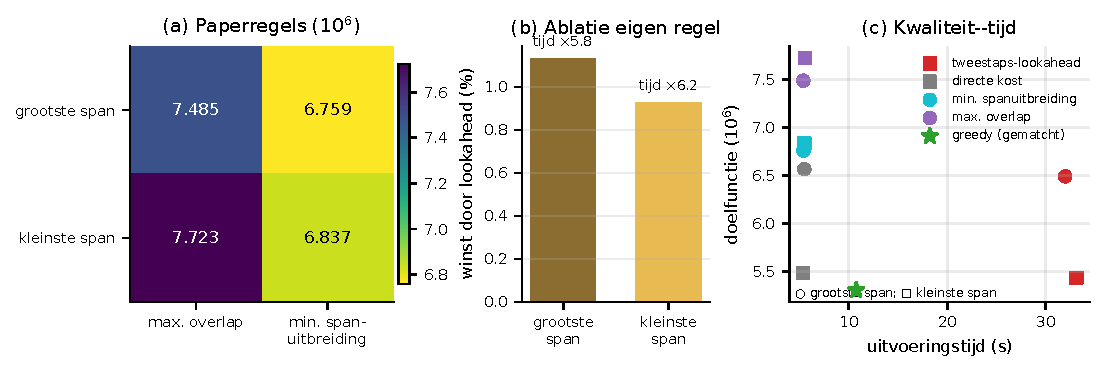
\includegraphics[width=0.82\linewidth]{figures/retrospective_seed.pdf}
\caption{De drie panelen tonen de doelfunctie van het oorspronkelijke
$2\times2$-ontwerp, de winst van de tweestapsvooruitblik en de mediane tijd met
IQR uit tien procesmetingen.}
\label{fig:app-seed}
\end{figure}
\endgroup


\end{document}
